\documentclass[12pt, a4paper, lithuanian]{article}
\usepackage[utf8x]{inputenc}
\def\LTfontencoding{L7x}
\PrerenderUnicode{ąčęėįšųūž}
\usepackage[\LTfontencoding]{fontenc}
\usepackage[lithuanian]{babel}
\usepackage{VUMIFPSkursinis}
\usepackage{cite}
\usepackage{amsmath}
\usepackage{bm}
\usepackage{amsfonts}
\usepackage{float}
\usepackage{graphicx}
\usepackage{color}
\usepackage{listings}
\usepackage{wrapfig}
\usepackage{algpseudocode}
\usepackage{algorithm}
\usepackage{algorithmicx}
\usepackage{caption}
\usepackage{subfig}


% Titulinio aprašas
\vumifdept{Programų sistemų katedra}
\vumifpaper{Kursinis darbas}
\title{Biojutiklio su selektyvia membrana kompiuterinis modeliavimas}
% \title{Esama situacija su dviem sluoksniais}
% \title{Ištirti selektyvios membranos įtaką amperometrinio bijojutiklio jautriui}
\def\titleineng{Computational modelling of biosensors with selective membrane}
\def\statusas{% Kai kurioms katedroms reikia nurodyti  
    4 kurso 1 grupės studentas \\
}
\author{
   Kęstutis Gimbutas
}

\supervisor{prof. dr. Romas Baronas}
\date{Vilnius – \the\year}

\begin{document}
\sloppy
\maketitle

\tableofcontents

\sectionnonum{Įvadas}
Biojutikliai yra analitiniai prietaisai, kurių pagrindinės sudedamosios dalys
yra biologinis darinys, kuris atpažįsta norimus cheminius junginius, ir
prietaisas, kuris to junginio atpažinimą  paverčia į elektros signalą. Elektros
signalo stiprumas yra proporcingas minėto cheminio elemento koncentracijai
nagrinėjamoje terpėje. Biojutikliai yra klasifikuojamini pagal įrenginio, kuris
paverčia vienos rūšies energiją kita,
prigimtį. Amperometriniai biojutikliai matuoja srovės stiprį faradais, kuri
kyla elektrode dėl biocheminės reakcijos produktų tiesioginės cheminės oksidacijos 
arba redukcijos. Kol matuojama srovė amperometriniuose biojutikliuose elektrodo potencialas yra
laikomas konstanta. Amperometriniai biojutikliai yra žinomi
kaip patikimi, pigūs ir reikšmingi medicinos, pramonės sritims
\cite{baronas2006computational}.

Praktiškas biojutiklis turi daugiasluoksnę fermento membraną. Elekrodas veikia
kaip biojutiklio rėlė, jis yra padengtas selektyviaja membrana po kurios seka
imobilizuotas fermentas. Selektyvioji membrana yra naudojama norint padidinti
biojutiklio selektyvumą \cite{baronas2006computational}. \\


*Kam to reikia, ka tai gali suteikti.

*Bus kuriamas modelis, tikrinama, ar galima jį skaitiškai aproksimuoti ir pan.

\section{Biojutiklio su selektyvia membrana modelis}
%Sudarant modelius bei lygtis buvo pasinaudota šaltiniais:
%\cite{baronas2009mathematical}, \cite{baronas2006computational},
%\cite{baronas2003influence}.

\subsection{Matematinis modelis}

Supaprastintas amperometrinis biojutiklis su seletyvia membrana turi tris
pagrindines sudedamąsias dalis: fermento sluoksnis($\Omega_2$),
selektyvios
membranos sluoksnis($\Omega_1$), elektrodas (žr. 1 pav.).
\begin{figure}[H]
    \centering
    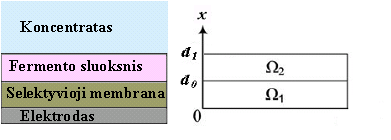
\includegraphics[scale=0.9]{img/modv1}
    \caption{Biojutiklio struktūra}
    \label{biojutiklio-struktura}
\end{figure}

Fermento sluoksnyje vyksta grįžtamoji cheminė reakcija, kurios metu (S)
, kuris supa biojutiklį,
susijungia su (E), kad suformuotų kompleksą (ES). Susiformavus minėtam
kompleksui jis pasidalija į reakcijos produktą (P) ir fermentą (E)
\cite{baronas2009mathematical}.  
\begin{equation}\label{eq:basic} 
    S + E \leftrightarrow ES \rightarrow E + P
\end{equation}

Selektyvios membranos sluoksnis yra skirtas atskirti (P) iš fermento sluoksnyje esančių
junginių. Dažniausiai tam yra naudojamos kietesnės ir didesnio tankio medžiagos
nei fermento sluoksnis, todėl selektyvios membranos ir (P) difuzinis
koeficientas yra mažesnis lyginant su (E) ir (S) arba (E) ir (P) difuziniais
koeficientais. Taip pat šis sluoksnis gali pagerinti kitas biojutiklio savybes kaip
tvirtumas, elekrodo ilgaamžiškumas. 

Junginiui (P) difuzijos būdu nukeliavus iki elektrodo įvyksta cheminė reakcija,
kurios pasakoje junginys (P) yra visiškai suvartojamas ir elektrode susidaro
elektros srovė. Daroma prielaida, kad šios reakcijos metu nesusidaro šalutiniai
produktai ir elektrodas nesidevi.

Remiantis supaprastinta schema tirpalas (S) prisijungia prie fermento (E)
ir yra
paverčiamas į produktą (P),
\begin{equation}\label{eq:basic}
    S \overset{E}{\rightarrow} P
\end{equation}

Uždaros sritys, kurios atitinka fermento ir selektyvios
membranos sluoksnius, atvaizduotos \ref{biojutiklio-struktura} pav.:
\begin{equation}
\begin{aligned}
    &\overline{\Omega}_1 = [0, d_0],\\
    &\overline{\Omega}_2 = [d_0, d_1]
\end{aligned}
\end{equation}

Tegu $\Omega_i$ yra atviros sritys atitinkačios uždarus regionus
$\overline{\Omega}_i$, i = 1, 2:
\begin{equation}
\begin{aligned}
    &\Omega_1 = (0, d_0),\\
    &\Omega_2 = (d_0, d_1)
\end{aligned}
\end{equation}

Srityje $\Omega_1$ vyksta tik produkto
difuzija, tuo tarpu $\Omega_2$ srityje vyksta fermento
reakcija su substratu ir jų transportavimas taip pat difuzija.

Apjungus fermento katalizuojamą reakciją fermento sluoksnyje su reakcijos
produkto (P) difuzija selektyviojoje membranoje ir su vienos
dimensijos erdvėje difuzija, kuri yra apibrėžta Ficko dėsniu, gautos šios
esminės lygtys ($0<t$):
\begin{equation}
\begin{aligned} 
    \label{eq:mat-modelis}
    &\frac{\partial P_1}{\partial t} = D_{1P} \frac{\partial^2 P_1}{\partial x^2}, \;
    \; x \in \Omega_1,\\
    &\frac{\partial S}{\partial t} = D_S \frac{\partial^2 S}{\partial x^2} -
    \frac{V_{max} S}{K_M + S},  \\ 
    &\frac{\partial P_2}{\partial t} = D_{2P} \frac{\partial^2 P_2}{\partial x^2} +
    \frac{V_{max} S}{K_M + S}, \; \; x \in \Omega_2 ,\;\; t > 0.\\
\end{aligned}
\end{equation}

Lygčių sistemoje (\ref{eq:mat-modelis}) x atitinka erdvę, o t – laiką, S(x, t)
yra koncentrato koncentracija, o P(x, t) yra reakcijos produkto koncentracija,
$\Omega_1$ – selektyvios membranos storis, $\Omega_2$ – fermento sluoksnio
storis, $V_{max}$ – maksimalus fermentacinis greitis, $ D_{1P}$, $ D_{2P}$, $ D_S$ - difuziniai medžiagų koeficientai, t - laikas nuo
simuliacijos pradžios, $ K_M$ - Michaelio konstanta. Michaelio konstanta $K_M$
nusako su kokios koncentracijos koncentratu yra pasiekiama pusė maksimalaus
reakcijos, kuri katalizuojama fermento, greičio.

\subsection{Pradinės ir kraštinės sąlygos}
Tegu x = 0 yra elektrodo paviršius, x = $d_1$ – riba tarp analizuojamo
tirpalo ir fermento membranos, o x = $d_0$ – riba tarp selektyviosios membranos
ir fermento sluoksnio. Iš pradžių nei (S) nei (P) nėra biosensorio
dalyse. Matavimai pradedami, kai koncentratas atsiduria ant fermento membranos
paviršiaus. Pradinėmis salygomis (t = 0) tikimasi:
\begin{equation}
\begin{aligned}
    &S(0,0) = 0, \\
    &S(x, 0) = 0,\; x \in \Omega_2,\\
    &S(d_1, 0) = S_0,
\end{aligned}
\end{equation}

\begin{equation}
\begin{aligned}
    &P_1(x, 0) = 0,\; x \in \overline\Omega_1,\\
\end{aligned}
\end{equation}

\begin{equation}
\begin{aligned}
    &P_2(x, 0) = 0,\; x \in \overline\Omega_2,\\
    &P_2(d_1, 0) = P_0.
\end{aligned}
\end{equation}

$S_0$ ir $P_0$ yra (S) ir (P) koncentracijos tiriamame tirpale. Dažniausiai
daroma prielaida, kad reakcijos produkto koncentracija tirpal yra lygi nuliui:
$P_0 = 0$. Taip pat, jeigu mišinys yra maišomas ir difuzijos sluoksnis (0 < x <
$d_1$) išlieka konstanta, daroma prielaida, kad fermento membranos paviršiuje
(x = $d_1$) substrato ir produkto koncentracijos išlieka konstanta. Iš to gauname fermento sluoksnio paviršiaus (x = $d_1$) kraštines salygas:
\begin{equation} 
    S(d_1, t) = S_0,\; t>0,
\end{equation}

\begin{equation} 
    P_2(d_1, t) = P_0 = 0,\; t>0.
\end{equation}

Reakcijos produkto koncentracija ant elektrodo paviršiaus (x = 0) visada
laikoma lygi nuliui dėl elektrodo poliarizacijos:
\begin{equation} 
    P_1(0,t)=0, \; t>0.
\end{equation}

Ant selektyviosios membranos paviršiaus (x = $d_0$) (S) nereguoja ir neprasiskverbia į
selektyviąją membraną, o (P) atvirkščiai – toliau skverbiasi link elektrodo
difuzijos pagalba. Nepaisant difuzijos koficientų ir kitų skirtumų tarp selektyvios ir
fermento membranų sluoksnių daroma prielaida, kad jų susilietimo taške abiejose
pusėse (P) koncentracija yra ta pati: P($\underset{y \to 0}{lim}(d_0 + y)$, t) =
P($\underset{y \to 0}{lim}(d_0 - y)$, t)  , iš to seka kraštinės sąlygos:
%\begin{equation} 
%    \left. D_S \frac{\partial S}{\partial x} \right|_{x=d_0} = 0, t>0.
%\end{equation}
\begin{equation} 
\begin{aligned}
    \left. D_S \frac{\partial S}{\partial x} \right|_{x=d_0} = 0, \;\;
    & \left. D_{1P} \frac{\partial P_1}{\partial x} \right|_{x=d_0} = 
    \left. D_{2P} \frac{\partial P_2}{\partial x} \right|_{x=d_0},\; t > 0 \\
    & P_1(d_0, t) = P_2(d_0, t),\; t>0.
\end{aligned}
\end{equation}

\section{Biojutiklio atsako charakteristikos}
\subsection{Biojutiklio srovė}

Fizikiniuose eksperimentuose išmatuota elektros srovė yra priimtinas
biojutiklio atsako kriterijus. Srovė yra tiesiogiai proporcinga elektrodo
plodui ir priklauso nuo elektroaktyvių medžiagų (P)
kiekio prie elektrodo paviršiaus (x = 0). Remiantis vienos dimensijos modeliu
ir pritaikius Faradėjaus ir Ficko dėsnius srovė dali būti apskaičiuota
remiantis formule:
\begin{equation}
    \label{eq:srove}
    \left. i(t) \approx n_eFD_{1P}\frac{\partial P}{\partial x} \right|_{x=0}.
\end{equation}

Formulėje (\ref{eq:srove}) $n_e$ yra elektronų skaičius, kurie dalyvavo srovės
keitime, F yra Faradėjaus konstanta, F = 96,485 C/mol.

Laikui artėjant į begalybę sistema įgauna pastobų būvį. I paimta, kaip jo
srovės rodiklis:
\begin{equation}
    I = \underset{t \to \infty}{lim} \ i(t)
\end{equation}

\subsection{Biojutiklio atsako laikas}

Laiko intervalas nuo vyksmo pradžios iki srovės išmatavimo momento yra
vadinamas biojutiklio atsako laiku. Amperometrinių biojutiklių, kurių modulis
yra stacionarus, atsako laikui išmatuoti dažniausiai naudojamas laikas, kurio
prireikia, kad srovės pokytis per nusistatytą laiko intervalą neviršytų
nusistatytos srovės vertės pokyčio. T – laikas, kurio reikia, kad pasiekti
mažesnį srovės pokyčio greitį, nei nusistatysasis $\epsilon$:
\begin{equation} 
\begin{aligned}
    T = \underset{i(t)>0}{min}\left\{t:\frac{t}{i(t)} \left| i'(t)
    \right| < \epsilon \right\}
    %  T = \underset{i(t)>0}{min}\left\{t:\frac{t}{i(t)} \left| \frac{\partial i(t)}{\partial t}
    % \right| < \epsilon \right\}
\end{aligned}
\end{equation}

Tačiau atsako laikas T, kaip apytikslis laikas biojutiklio pastovaus laiko
įvertis, yra labai jautrus nusistatytam neviršijamam srovės pokyčio greičiui
$\epsilon$, kai $\epsilon \to 0$, tada $T \to \infty$. Todėl yra naudojamas
dalinai pastovios srovės laikas.  
 
\section{Biojutiklio matematinio modelio skaitinis aproksimavimas}
\subsection{Neišreikštinė schema}

\begin{equation}
\begin{aligned} 
    &\frac{S_i^{j+1} - S_i^j}{\tau} = D_S\frac{S_{i+1}^{j+1} -
    2S_i^{j+1} + S_{i-1}^{j+1}}{h^2} -
    \frac{V_{max} S_i^j}{K_M + S_i^j},\;i = k,\;...,\;N-1\\ 
    &\frac{P_i^{j+1} - P_i^j}{\tau} = D_{2P}\frac{P_{i+1}^{j+1} -
    2P_i^{j+1} + P_{i-1}^{j+1}}{h^2} +
    \frac{V_{max} S_i^j}{K_M + S_i^j},\;i = k,\;...,\;N-1\\ 
    &\frac{P_i^{j+1} - P_i^j}{\tau} = D_{1P}\frac{P_{i+1}^{j+1} -
    2P_i^{j+1} + P_{i-1}^{j+1}}{h^2}, \;i = 1,\;...,\;k-1\\ 
    &j=0,\;...,\;M-1.
\end{aligned}
\end{equation}

% \subsubsection{Pradinės ir kraštinės modelio sąlygos}
% \begin{equation}
% \begin{aligned}
%     &S_i^0 = 0, i = 0,\;...,\;N-1,\\
%     &S_N^0 = S_0,
% \end{aligned}
% \end{equation}
% 
% \begin{equation}
% \begin{aligned}
%     &P_i^0 = 0, i = 0.\;...,\;N-1,\\
%     &P_N^0 = P_0
% \end{aligned}
% \end{equation}
% 
% \begin{equation} 
%     S_0^j = S_1^j, S_N^j = S_0, j=1,\; ...,\;M, 
% \end{equation}
% 
% \begin{equation} 
%     P_0^j = 0, P_N^j = P_0, j=1,\; ...,\;M, 
% \end{equation}
% 
\subsection{Skaičiavimo procedūra}

\begin{equation} 
    i(t_j) \approx t_j = n_eFD_pP_i^j/h,\; j=1,\;...,\;M. 
\end{equation}

\section{Skaitinio sprendimo tikrinimas}
\subsection{Pradinės skaičiavimų sąlygos}
 
 \begin{equation}
 \begin{aligned}
     &S_0 = 1 \mathrm{\mu M},\; P_0 = 0 \mathrm{\mu M},\\
     &D_s = 300 \mathrm{\mu m^2/s},\; D_{2p} = 300 \mathrm{\mu m^s/s}, D_{1p} = 300 \mathrm{\mu m^s/s},\\\
     &d_0 = 10\ \mathrm{\mu m},\; d_1 = 10 \mathrm{\mu
 m},\ 15 \mathrm{\mu m},\ 100 \mathrm{\mu m},\ 150\mathrm{\mu m},\;\\
     &\tau = 0.1\mathrm{s},\; h=0.1 \mathrm{\mu m},\\
     &V_{max} = 100\mathrm{\mu M /s},\; \epsilon = 0.05,\\
     &F=961485,\; K_M= 100\mathrm{\mu M},\; n_e = 2.
 \end{aligned}
 \end{equation}
 
\subsection{Gautos matricos iš neišreikštinės schemos}
\textit{Lygčių sistemos gautos naudojant baigtinių skirtumų metodą ir neišreikštines
schemas. Lygtys išspręstos taikant triįstrižainių matricų algoritmą. Laiko
žingsnis - $\tau$ (indeksas $j$), erdvės žingsnis - $h$ (indeksas $i$).}
\begin{equation}
\left\{
\begin{aligned}
    &S_{i+1}^{j+1}-S_i^{j+1}\left(1+\frac{h^2}{D_S\tau}\right)
= \frac{h^2}{D_S\tau} \left(\frac{V_{max}S_i^j\tau}{K_M+S_i^j}-S_i^j\right),\; \;
i = k +1,\\
    &\dots\;,\\
    &S_{i-1}^{j+1}-S_i^{j+1}\left(2+\frac{h^2}{D_S\tau}\right)+S_{i+1}^{j+1}
        = \frac{h^2}{D_S\tau}
        \left(\frac{V_{max}S_i^j\tau}{K_M+S_i^j}-S_i^j\right),\; \; i =
        k +2,\;...,\;N-1,\\
    &\dots\;,\\
    &S_0 + S_{i-1}^{j+1} - S_i^{j+1}\left(2+\frac{h^2}{D_S\tau}\right)
        =  \frac{h^2}{D_S\tau}
    \left(\frac{V_{max}S_i^j\tau}{K_M+S_i^j}-S_i^j\right),\; \; i = N.
\end{aligned}
\right.
\end{equation}

\begin{equation}
\left\{
\begin{aligned}
%    &P_{i+1}^{j+1}-P_i^{j+1}\left(2+\frac{h^2}{D\tau}\right)
%    = \frac{h^2}{D\tau} \left(-P_i^j -\frac{V_{max}S_i^j\tau}{K_M+S_i^j}\right),\; \; i = 1,\\
    &P_{i+1}^{j+1}-P_i^{j+1}\left(2+\frac{h^2}{D_{1P}\tau}\right)
    = -\frac{h^2}{D_{1P}\tau} P_i^j,\; \; i = 1,\\
    &\dots\;,\\
%    &P_{i-1}^{j+1}-P_i^{j+1}\left(2+\frac{h^2}{D\tau}\right)+P_{i+1}^{j+1}
%        = \frac{h^2}{D\tau}
%    \left(\frac{V_{max}S_i^j\tau}{K_M+S_i^j}-S_i^j\right),\; \; i =
%        2,\;...,\;k-1,\\
    &P_{i-1}^{j+1}-P_i^{j+1}\left(2+\frac{h^2}{D_{1P}\tau}\right)+P_{i+1}^{j+1}
    =-\frac{h^2}{D_{1P}\tau} P_i^j,\; \; i = 2,\;...,\;k,\\
    &P_{i-1}^{j+1}-P_i^{j+1}\left(2+\frac{h^2}{D_{2P}\tau}\right)+P_{i+1}^{j+1}
    = \frac{h^2}{D_{2P}\tau}
    \left(\frac{V_{max}S_i^j\tau}{K_M+S_i^j}-P_i^j\right),\; \; i =
        k +1,\;...,\;N-1,\\
    &\dots\;,\\
    &P_0 + P_{i-1}^{j+1} - P_i^{j+1}\left(2+\frac{h^2}{D_{2P}\tau}\right)
        =  \frac{h^2}{D_{2P}\tau}
        \left(\frac{V_{max}S_i^j\tau}{K_M+S_i^j}-P_i^j\right),\; \; i = N.
\end{aligned}
\right.
\end{equation}

\subsection{Rezultatai}
 \begin{figure}[H]
     \centering
     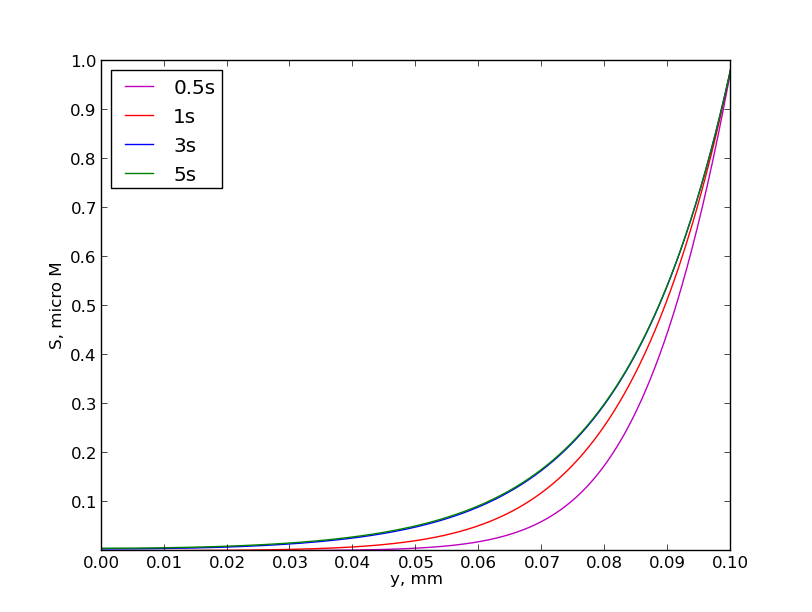
\includegraphics[scale=0.5]{img/kurS}
     \caption{Koncentratas $\Omega_2$ srityje}
     \label{img:mlp}
 \end{figure}
 
 \begin{figure}[H]
     \centering
     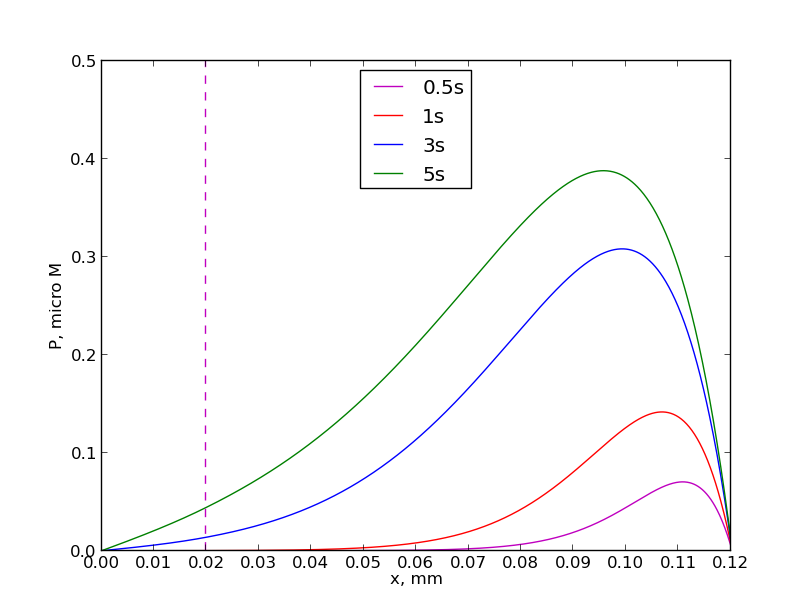
\includegraphics[scale=0.5]{img/kurP}
     \caption{Produktas $\Omega_1$ ir $\Omega_2$ srityse}
     \label{img:mlp}
 \end{figure}
 
 \begin{figure}[H]
     \centering
     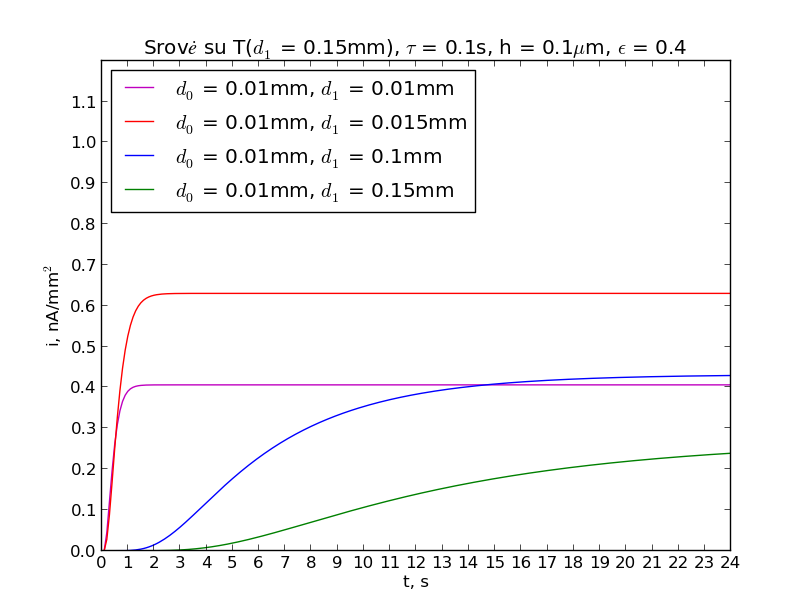
\includegraphics[scale=0.5]{img/kurI}
     \caption{Srovė, kai $\Omega_1 = d_0$ ir $\Omega_2 = d_1$}
     \label{img:mlp}
 \end{figure}

\sectionnonum{Rezultatai ir išvados} 
Remiantis barono knyga buvo sudarytas matematinis modelis

Pasiulytas matematinio modelio skaitinis aproksimavimo metodas
pasiulytas skaitinio aproksimavimo medotas istestuotas
Programisai realizuotas pasiulytasis skaitinio aproksimavimo metodas
Patikrintas pasiulytasis skaitinio aproskimavimo metodas

Ateities darbai: galima nustatyti optimalias biojutiklio parametrus konkretiems
tirpalams; Praplesti matematini modeli, kad jis tenkintu platesnes salygas.

%\appendix
 
% \begin{figure}[H]
%     \centering
%     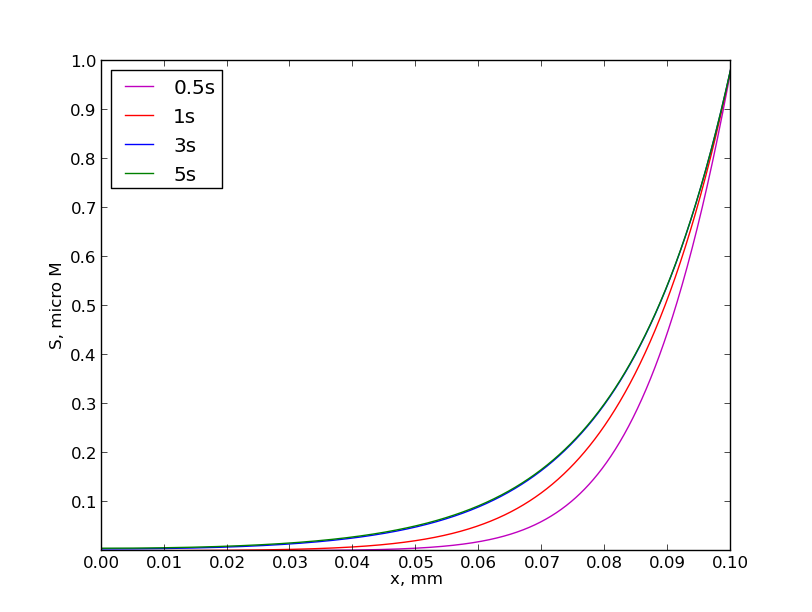
\includegraphics[scale=0.5]{img/S}
%     \caption{Substrate}
%     \label{img:mlp}
% \end{figure}
% 
% \begin{figure}[H]
%     \centering
%     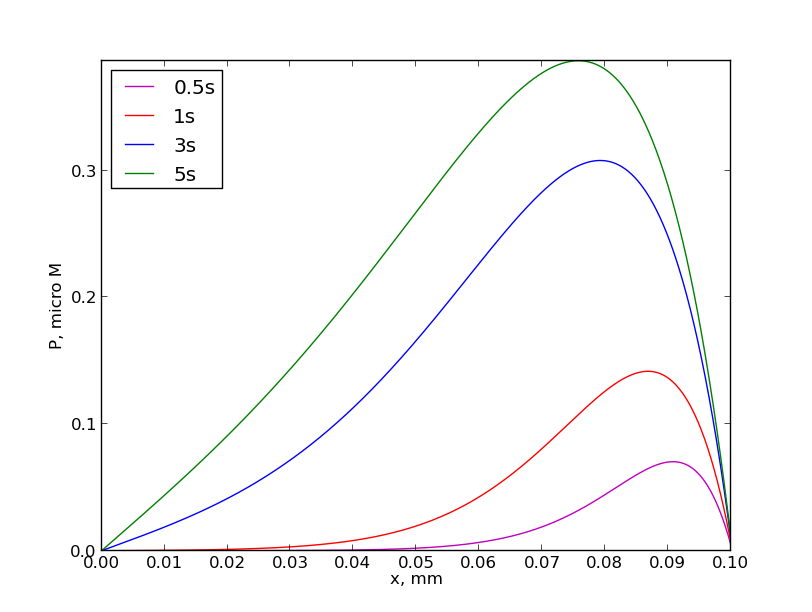
\includegraphics[scale=0.5]{img/P}
%     \caption{Product}
%     \label{img:mlp}
% \end{figure}
% 
% \begin{figure}[H]
%     \centering
%     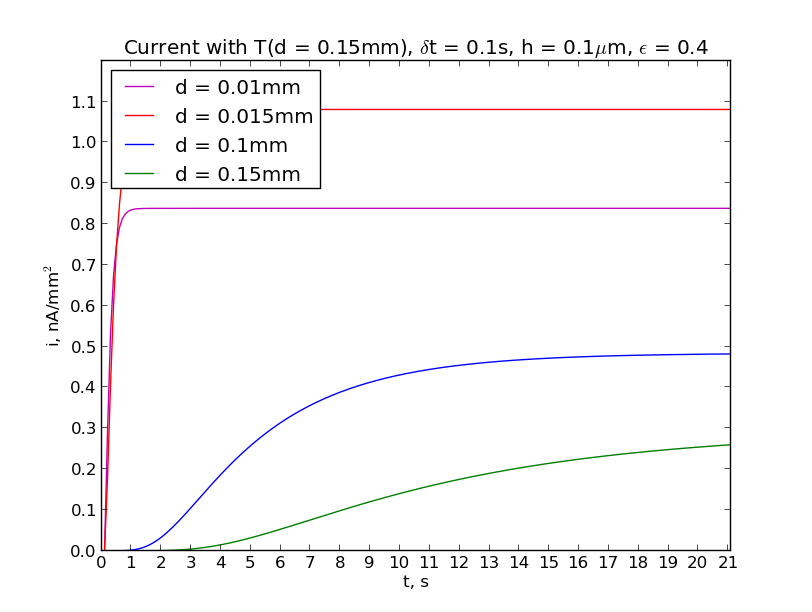
\includegraphics[scale=0.5]{img/i}
%     \caption{Current}
%     \label{img:mlp}
% \end{figure}
% 
%\appendix
%----------------------------------------------------

\bibliography{bibliografija}


%\appendix
%\section{Papildomų eksperimentų rezultatų lentelės}
%\begin{figure}[H]
%    \centering
%    \includegraphics[scale=0.5]{img/MLP}
%    \caption{Paveikslėlio pavyzdys}
%    \label{img:mlp}
%\end{figure}
%
\end{document}
